\section{Approach and Implementation}
This work builds upon the CAKE (sch\_cake) queuing discipline, with a particular focus on its bandwidth shaper. CAKE implements Active Queue Management (AQM) and rate limiting during packet dequeue, effectively eliminating the need for a backpressure mechanism. Through its bandwidth shaper, CAKE enforces a global rate limit on egress network traffic, preventing excessive packet buffering in the lower layers of the network stack. However, CAKE suffers from the aforementioned contention of the root qdisc lock, which prevents it from exploiting the potential of multiple transmission queues.

\subsection{Approach}
This work overcomes the aforementioned shortcomings by enabling a scalable version of \textit{sch\_cake}~\cite{cake} to run in combination with the MQ qdisc.
%
This multi-queue version of CAKE is referred to as \textit{mq-cake}.
In order to improve scalability and correctly enforce a global rate limit a synchronization mechanism between installed \textit{mq-cake} instances is necessary.
%
By synchronizing at regular intervals, \textit{mq-cake} instances estimate their local rate limit based on their sibling \textit{mq-cake} instances' activity.  
%
This rate estimation is implemented in a way that avoids any lock- or atomic operations as a means of achieving optimal scalability.
%

The synchronization frequency determines how fast a qdisc can react to changes in the activity of its sibling qdiscs.
If this frequency is higher, the local rate limit is able to converge more quickly to the correct value but the CPU load also increases.
When this frequency is lower, the CPU load decreases but takes longer to converge.
%
Further, the CPU load increases as the number of hardware queues grows, since more data structures must be accessed in order to estimate the local rate.
%
However, if the per-packet CPU load becomes too high, the achieved throughput lowers, potentially hindering the system from driving higher rate limits.
This phenomenon will be covered in greater detail in Chapter~\ref{sec:evaluation}.

\begin{figure}[h]
    \centering
    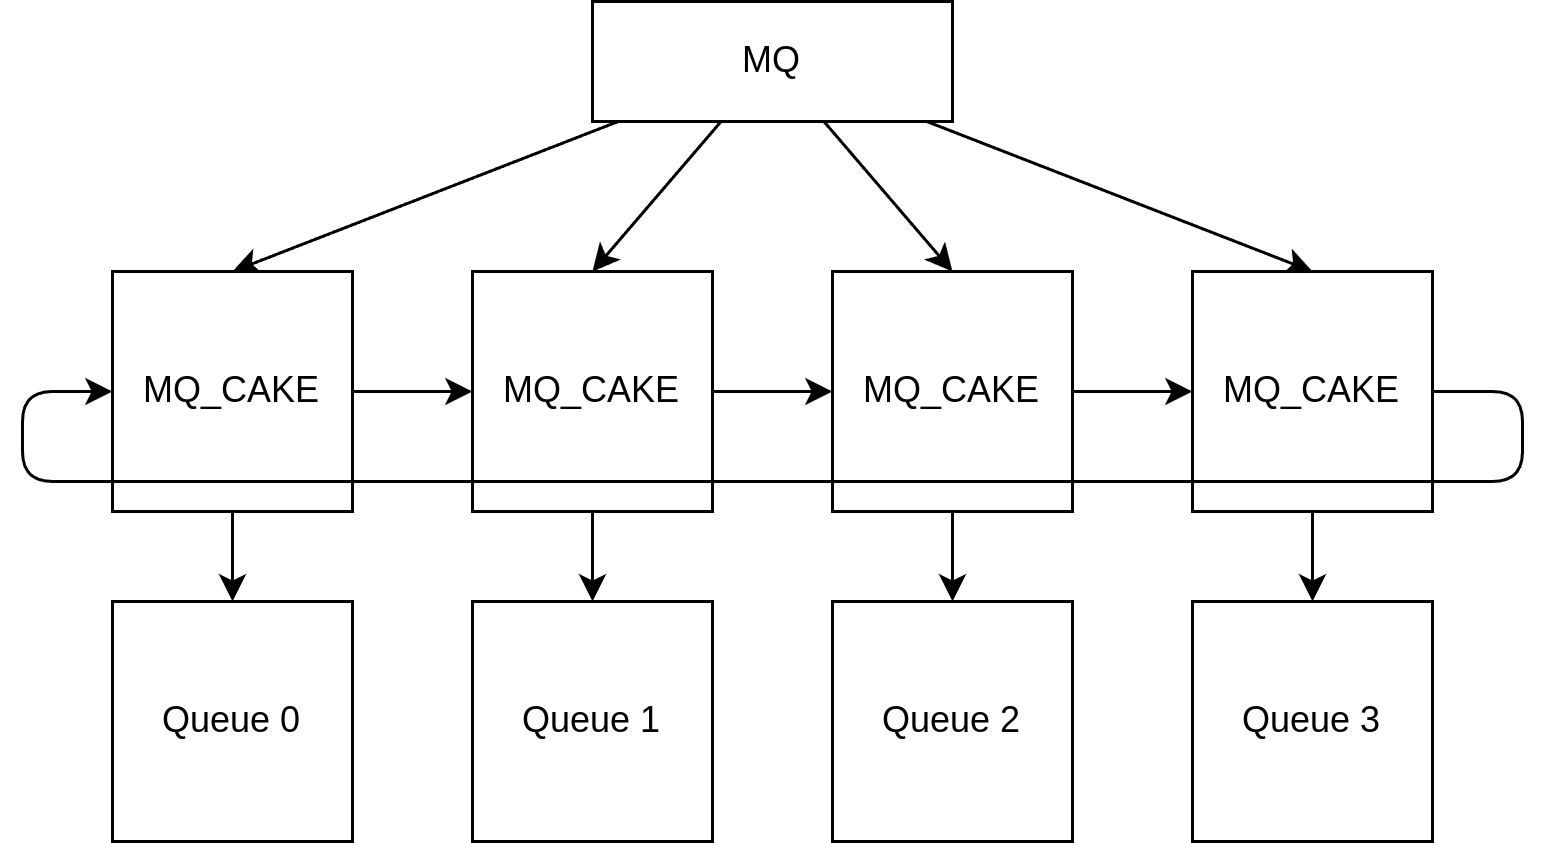
\includegraphics[scale=0.15]{images/mq_cake_architecture.drawio.png}
    \caption{mq-cake architecture with four hardware transmission queues}\label{fig:mq_cake_architecture}
\end{figure}

\subsection{Implementation}
Central to this synchronization mechanism is a linked list between all \textit{mq-cake} instances installed on a network interface.
%
During the installation process of a new \textit{mq-cake} instance, this new instance searches for sibling qdiscs and adds itself to their linked list.
%
Figure~\ref{fig:mq_cake_architecture} shows an example of the proposed architecture for four hardware queues.
This approach relies on estimating how many instances of \textit{mq-cake} are actively sending packets --- these instances are referred to as either \textit{active queues} or \textit{active qdiscs}.
%
According to this number, a \textit{mq-cake} instance determines its local rate limit by dividing the global rate limit by the number of active \textit{mq-cake} qdiscs.
%
\begin{align}
    \text{local rate limit} = \frac{\text{global rate limit}}{\text{number of active qdiscs}}
\end{align} 

Once the qdisc is installed, each \textit{mq-cake} instance scans the list of siblings in regular intervals to count the number of active qdiscs. 
%
This duration of this interval is called the synchronization time, or \textit{synctime} for short.
%
If the \textit{synctime} is set too low, the overhead caused by the qdisc scan increases, lowering the achievable throughput and thus decreasing the maximum enforceable rate limit.
The lower bound depends on the time it takes to complete one scan of all sibling qdisc.
If this value is set too high, the accuracy suffers due to the slower convergence to the correct local rate estimation.
%
In particular, this occurs if a qdisc's state changes either from active to inactive or vice versa.
%
The default setting for this value is $200\mu s$, which is an appropriate value to ensure fast convergence and low CPU overhead. 
%

A scanning instance considers another qdisc active if it has packets enqueued and/or has sent packets since the last scan.
%
The logic behind these metrics is demonstrated in the following two scenarios:
%
(1) If a qdisc has only large packets enqueued while the global rate limit is low, the inter-packet gap may be larger than the \textit{synctime}.
This is due to fact that qdiscs with large packets are slower in their release time and are buffered in the qdiscs queue.
%
This scenario would lead the qdisc to falsely read the instance as inactive if only considering the \textit{packet sent} metric, as the number of sent packets between the two scans  would not have changed.
%
However, any qdisc with packets enqueued is active, as it will eventually dequeue them and use its portion of the configured rate limit.
%
(2) If a qdisc receives very small packets while the global rate limit is high, the backlog of a qdisc consistently remains empty, as packets are less likely to be buffered and thus are immediately sent out.
%
This scenario would also lead the qdisc to falsely read the instance as inactive if only considering the \textit{has packets backlogged} metric, since the packets are only buffered for a very short interval.
%
Thus, the scanning qdisc needs to maintain a counter --- similar to a heartbeat signal --- to determine if another qdisc has sent packets since the last synchronization scan.
%

This external qdisc observation is necessary because a qdisc cannot mark itself as (in)active, as its code is only executed if the qdisc receives a packet or is triggered by a timer.
%
If a qdisc runs empty of packets and there are no further packets enqueued, the qdisc can no longer change its status as active or inactive.
%
This means that, should a qdisc run empty, it would need to mark itself as inactive; but in cases where packets are immediately sent out, the qdisc would oscillate
between active and inactive, leading to inaccurate values for other qdiscs. 
%

The two activity metrics are read and written using the READ/WRITE\_ONCE macros.
%
Thus, the reads and writes are racy --- however, this does not present a problem, as the activity metrics do not rely on exact values but rather on whether the backlog of a qdisc is zero and whether the number of sent packets has changed.
%
This approach has the benefit of not building contention points while still achieving accurate local rate limit estimations.
%
Algorithm~\ref{alg:algo} shows this synchronization algorithm.
%
The source code of \textit{MQ\_CAKE} is published here: \url{https://github.com/mq-cake/linux-mq-cake}.

\begin{algorithm}[h]
    \caption{Synchronization algorithm}\label{alg:algo}
\begin{algorithmic}[1]
\Procedure{get\_active\_queues}{}
\If{now - last\_interval $<$ SYNC\_INTERVAL}
    \State \Return -1;
\EndIf
\State active\_queues = 1;
\ForAll{$q$ in qdisc\_list}
    \If{$q$ has packets backlogged}
    \State active\_queues++;
    \ElsIf{$q$ has sent packets since last interval}
    \State active\_queues++;
    \EndIf
\EndFor
\State last\_interval = now
\State \Return active\_queues;
\EndProcedure
\end{algorithmic}
\end{algorithm}
